\documentclass{subfiles}
\begin{document}
    \begin{figure}[!h]
        \centering
        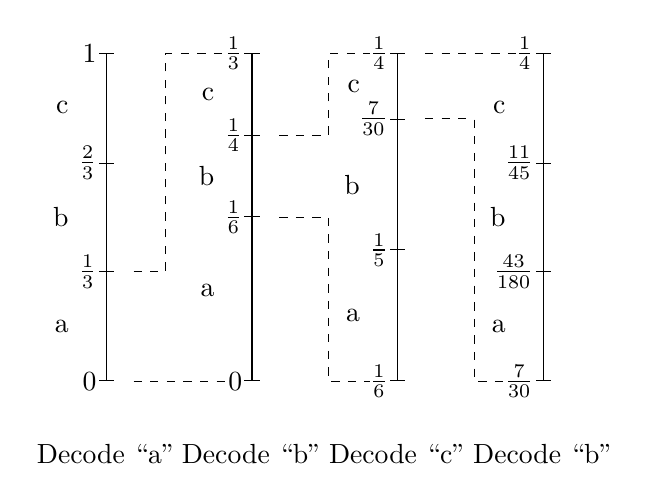
\begin{tikzpicture}[scale=0.925]

            % Step 1: read "a"
            % Equally probable symbols
            %% Ranges
            \draw [ |- ] (0, 0) -- (0, 1.5);
            \draw [ |-| ] (0, 1.5) -- (0, 3);
            \draw [ -| ] (0, 3) -- (0, 4.5);

            %% Symbols 
            \node at (-0.25, 0.75) [label=left:a] {};
            \node at (-0.25, 2.25) [label=left:b] {};
            \node at (-0.25, 3.75) [label=left:c] {};

            %% Probabilities
            \node at (0, 0) [anchor=east] {\(0\)};
            \node at (0, 1.5) [anchor=east] {\(\frac{1}{3}\)};
            \node at (0, 3) [anchor=east] {\(\frac{2}{3}\)};
            \node at (0, 4.5) [anchor=east] {\(1\)};

            %% Update probabilities
            \node at (0, -1) {Decode ``a''};

            %% Range selection
            \draw [dashed] (0.375, 0) -- (1.635, 0);
            \draw [dashed] (0.375, 1.5) -- (0.8125, 1.5) -- (0.8125, 4.5) -- (1.625, 4.5);

            % Step 2: read "b"
            % Update probabilities
            %% Ranges
            \draw [ |- ] (2, 0) -- (2, 2.25);
            \draw [ |-| ] (2, 2.25) -- (2, 3.375);
            \draw [ -| ] (2, 3.375) -- (2, 4.5);

            %% Symbols
            \node at (1.75, 1.25) [label=left:a] {};
            \node at (1.75, 2.8125) [label=left:b] {};
            \node at (1.75, 3.9375) [label=left:c] {};

            %% Probabilities
            \node at (2, 0) [anchor=east] {\(0\)};
            \node at (2, 2.25) [anchor=east] {\(\frac{1}{6}\)};
            \node at (2, 3.375) [anchor=east] {\(\frac{1}{4}\)};
            \node at (2, 4.5) [anchor=east] {\(\frac{1}{3}\)};

            %% Update probabilities
            \node at (2, -1) {Decode ``b''};

            %% Range selection
            \draw [dashed] (2.375, 2.25) -- (3.05, 2.25) -- (3.05, 0) -- (3.625, 0);
            \draw [dashed] (2.375, 3.375) -- (3.05, 3.375) -- (3.05, 4.5) -- (3.625, 4.5);

            % Step 3: read "c"
            % Update probabilities
            %% Ranges
            \draw [ |- ] (4, 0) -- (4, 1.8);
            \draw [ |-| ] (4, 1.8) -- (4, 3.6);
            \draw [ -| ] (4, 3.6) -- (4, 4.5);

            %% Symbols
            \node at (3.75, 0.9) [label=left:a] {};
            \node at (3.75, 2.7) [label=left:b] {};
            \node at (3.75, 4.05) [label=left:c] {};

            %% Probabilities
            \node at (4, 0) [anchor=east] {\(\frac{1}{6}\)};
            \node at (4, 1.8) [anchor=east] {\(\frac{1}{5}\)};
            \node at (4, 3.6) [anchor=east] {\(\frac{7}{30}\)};
            \node at (4, 4.5) [anchor=east] {\(\frac{1}{4}\)};

            %% Update probabilities
            \node at (4, -1) {Decode ``c''};

            %% Range selection
            \draw [dashed] (4.375, 3.6) -- (5.05, 3.6) -- (5.05, 0) -- (5.625, 0);
            \draw [dashed] (4.375, 4.5) -- (5.625, 4.5);

            % Step 4: read "d"
            % Update probabilities
            %% Ranges
            \draw [ |- ] (6, 0) -- (6, 1.5);
            \draw [ |-| ] (6, 1.5) -- (6, 3);
            \draw [ -| ] (6, 3) -- (6, 4.5);

            %% Symbols
            \node at (5.75, 0.75) [label=left:a] {};
            \node at (5.75, 2.25) [label=left:b] {};
            \node at (5.75, 3.755) [label=left:c] {};

            %% Probabilities
            \node at (6, 0) [anchor=east] {\(\frac{7}{30}\)};
            \node at (6, 1.5) [anchor=east] {\(\frac{43}{180}\)};
            \node at (6, 3) [anchor=east] {\(\frac{11}{45}\)};
            \node at (6, 4.5) [anchor=east] {\(\frac{1}{4}\)};

            %% Update probabilities
            \node at (6, -1) {Decode ``b''};
        \end{tikzpicture}
        \caption{Step by step decoding of \(0.2416\) via the adaptive \gls{ac}.}
        \label{Fig:7}
    \end{figure}
\end{document}
